\section{Formal Analysis Using Alloy}
In this section, the formal analysis and modeling of the system that was performed using Alloy shall be represented. The analysis has been performed with a focus on the various data flows of the system. Since, the core abstract goal of the system is the aggregation and communication of data to different parties; such as the communication of accident reports to authorities, or the communication of insights such as area safety and other statistics to both users and authorities; the data flows were our main concern in this formal analysis. As such, the bidirectional data flow between the system and the authorities has been modeled, as well as, the generation of data by the users in the form of violation reports all the while ensuring the consistency constraints; such as the fact that no report may be created by more than one user. Moreover, this analysis models other critical aspects ensuring the valid operation of the system such as the registration process and the fact that no two users may have a duplicate username or fiscal code or that all users have performed a registration.

	\lstinputlisting{alloy-final.als}
	
	\begin{figure}[H]	
		\centering
		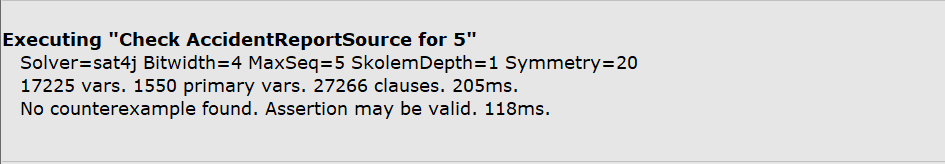
\includegraphics[scale=0.6]{images/ReportSourceAssertion.png}
		\caption{Result of Accident Report Source Assertion}
	\end{figure}
	
	\begin{figure}[H]	
		\centering
		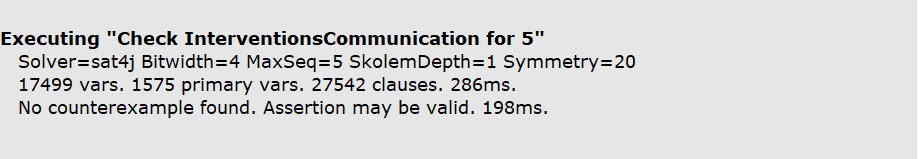
\includegraphics[scale=0.6]{images/InterventionCommAssertion.png}
		\caption{Result of Intervention Communication Assertion}
	\end{figure}	
		
In the above figures, the results of the assertions on accident reports and interventions are shown; these assertions were performed to ensure, first, the fact that accident reports come from authorities since the system is not able to produce with accident reports without such communication from the municipality through the agreed-upon data channels and to ensure that interventions are communicated to the authorities, this is due to the fact that the only motivation for the formulation of interventions by the system is to be communicated to the authorities.
	
	\begin{figure}[H]	
		\centering
		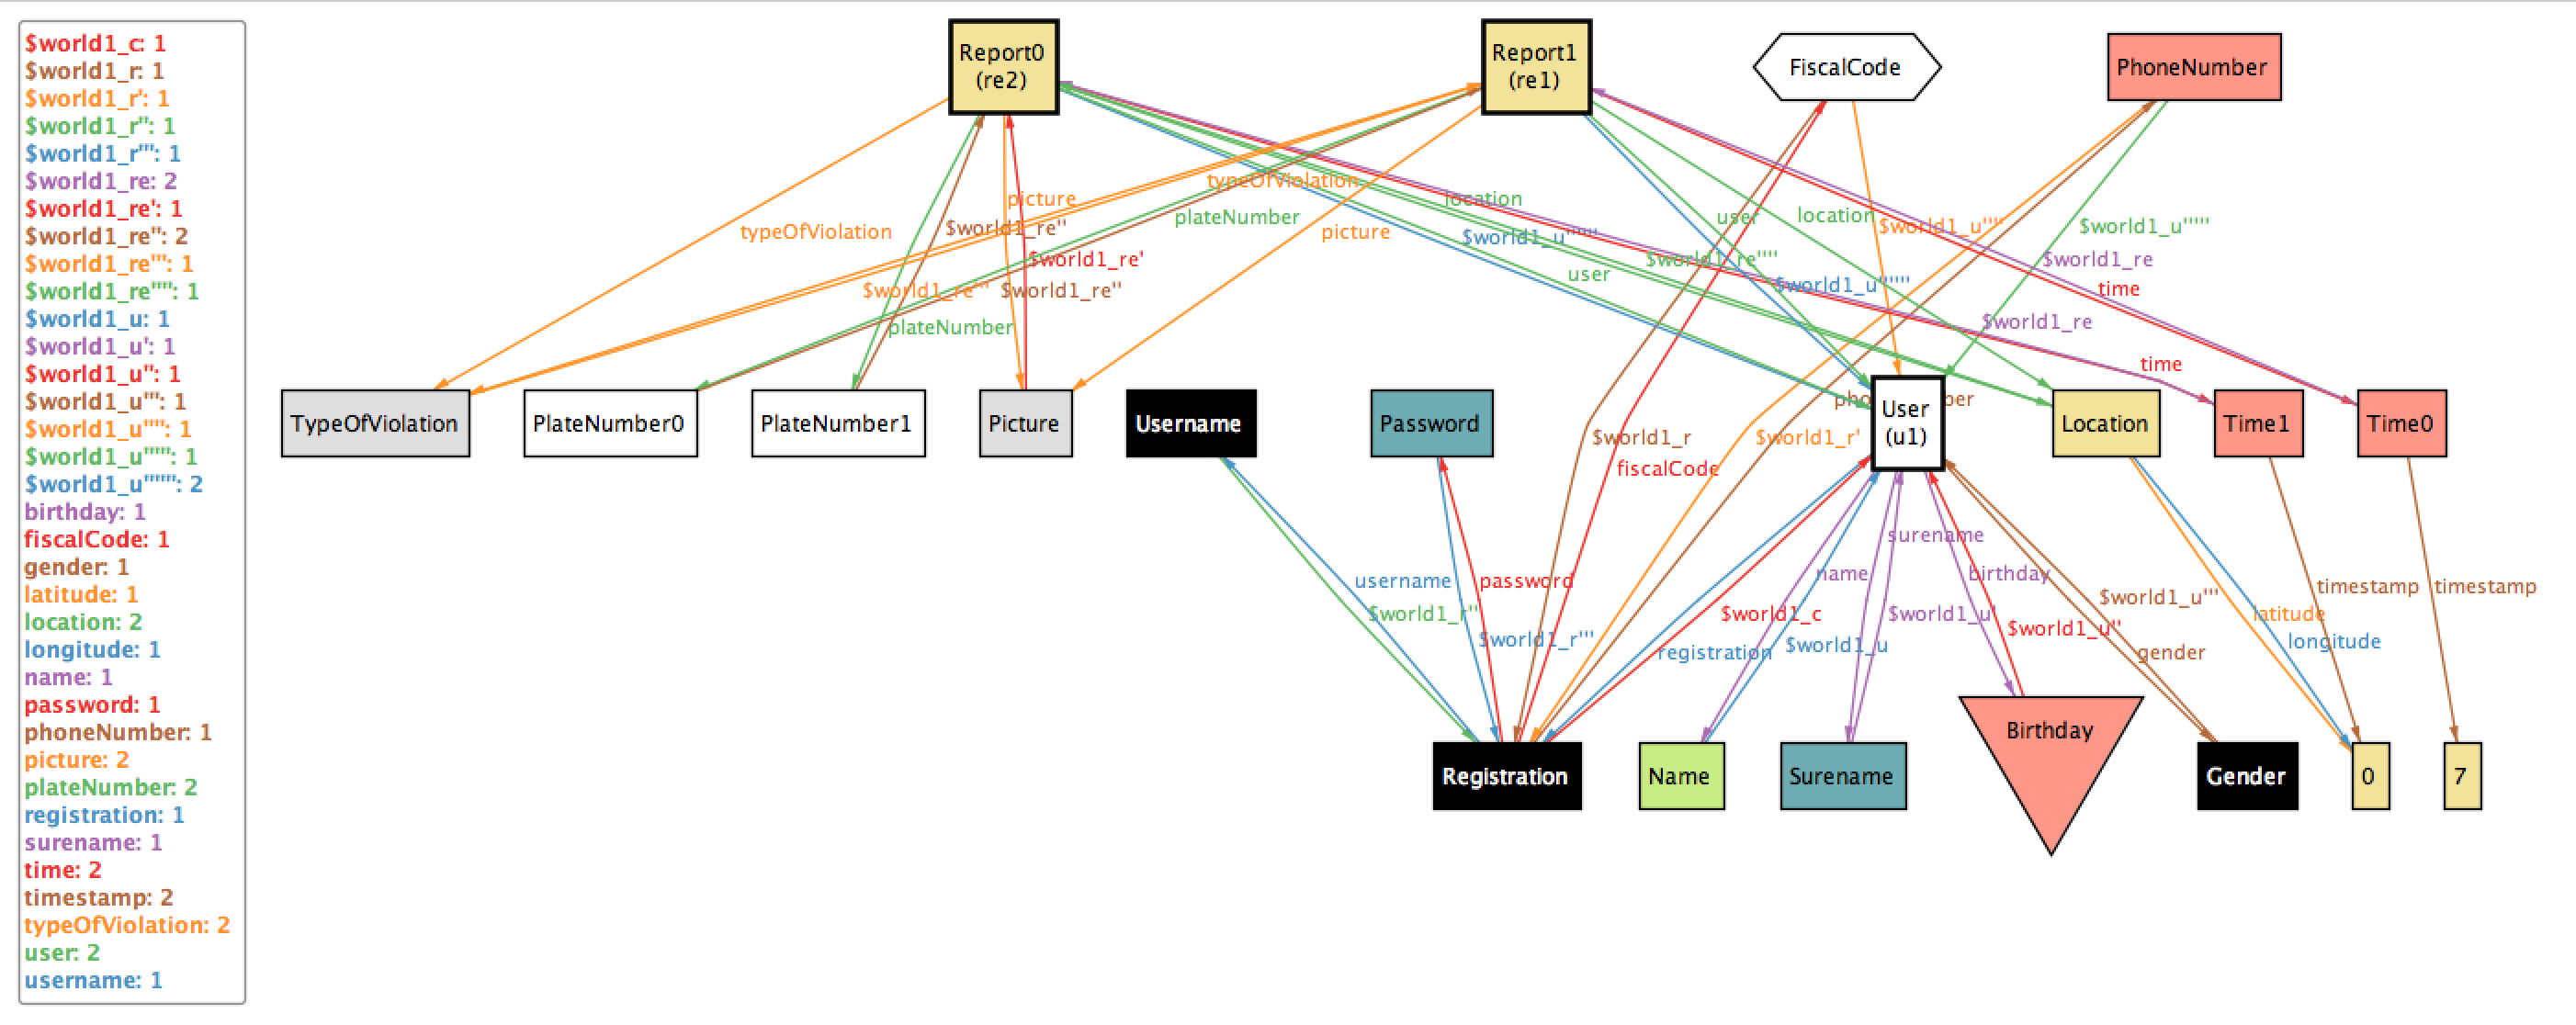
\includegraphics[scale=0.35]{images/World1.png}
		\caption{World One generated by Alloy Analyzer 4.2}
	\end{figure}
	
The above world created by the Alloy Analyzer shows the overall consistency of the model focusing specifically on the users and the reports; in the sense that, all critical aspects of the system are modeled in a valid way. In example, all users have one and only one registration with a unique username and fiscal code, all reports are created by a unique user and that all reports have a location, time, plate number and an image of the violation in them.	
	
	\begin{figure}[H]	
		\centering
		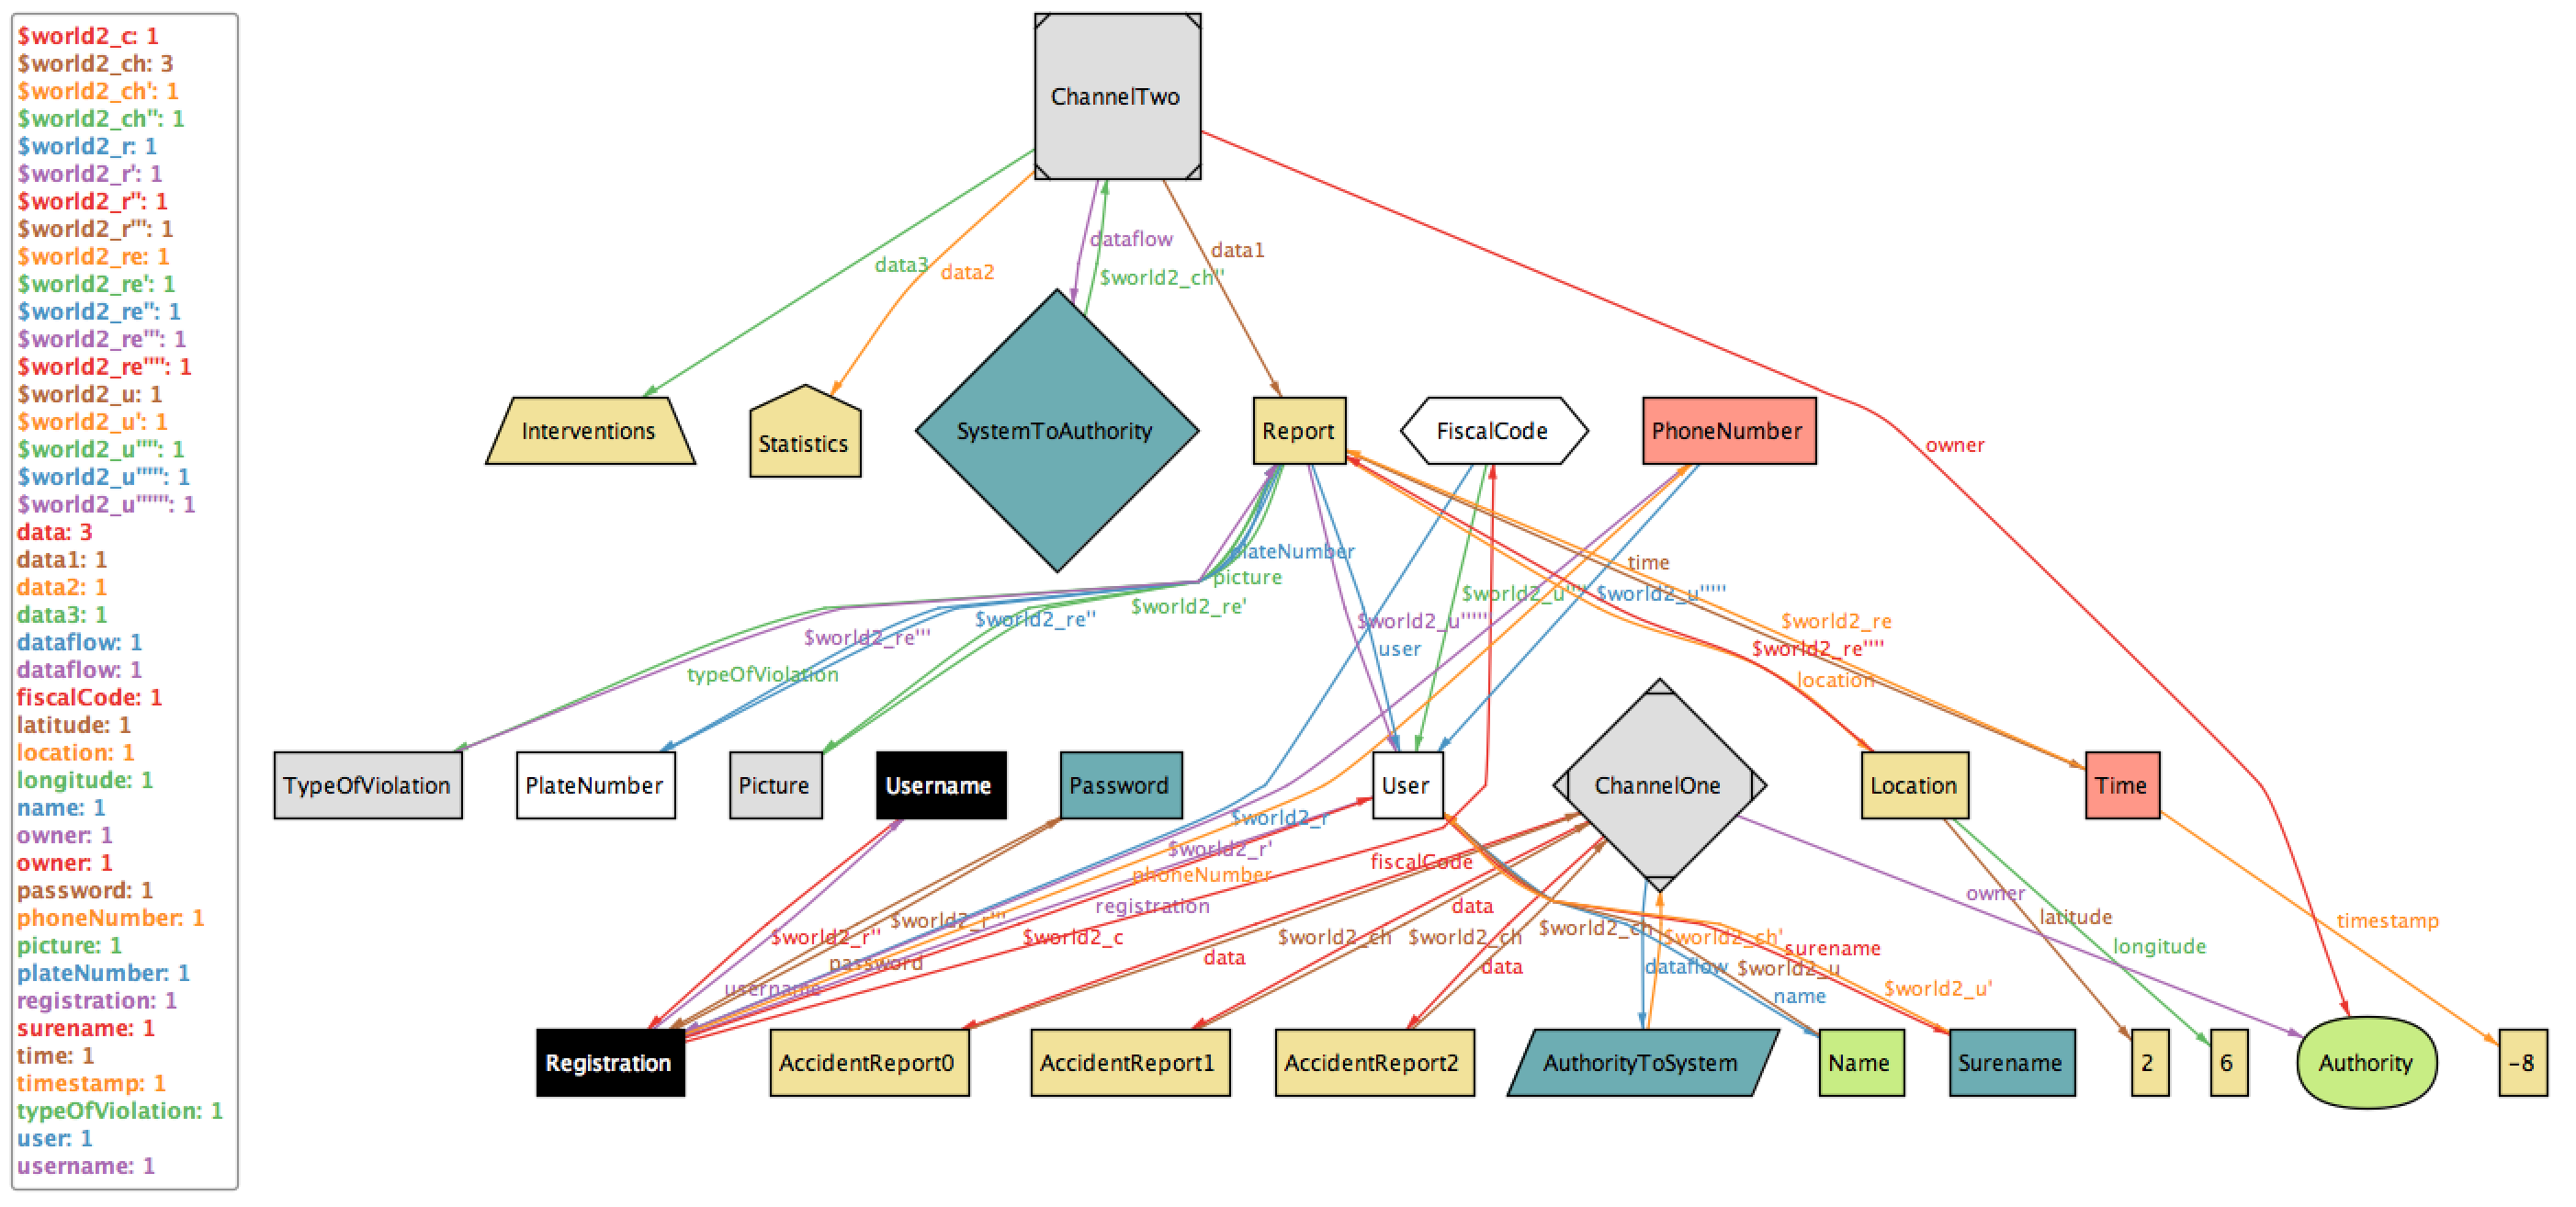
\includegraphics[scale=0.35]{images/World2.png}
		\caption{World Two generated by Alloy Analyzer 4.2}
	\end{figure}
	
World two shown in the above figure focuses on the consistency of the authority communication; modeling, the communication channels, their data flows and the authority that owns them. As well as, modeling the flow of accident reports from the authorities to the system. It can be seen that all accident reports reach the system through a data channel which is owned by a unique authority as it has been checked in the ReportSource assertion and that interventions are linked to a data channel from the system to the authority.
	
	\begin{figure}[H]	
		\centering
		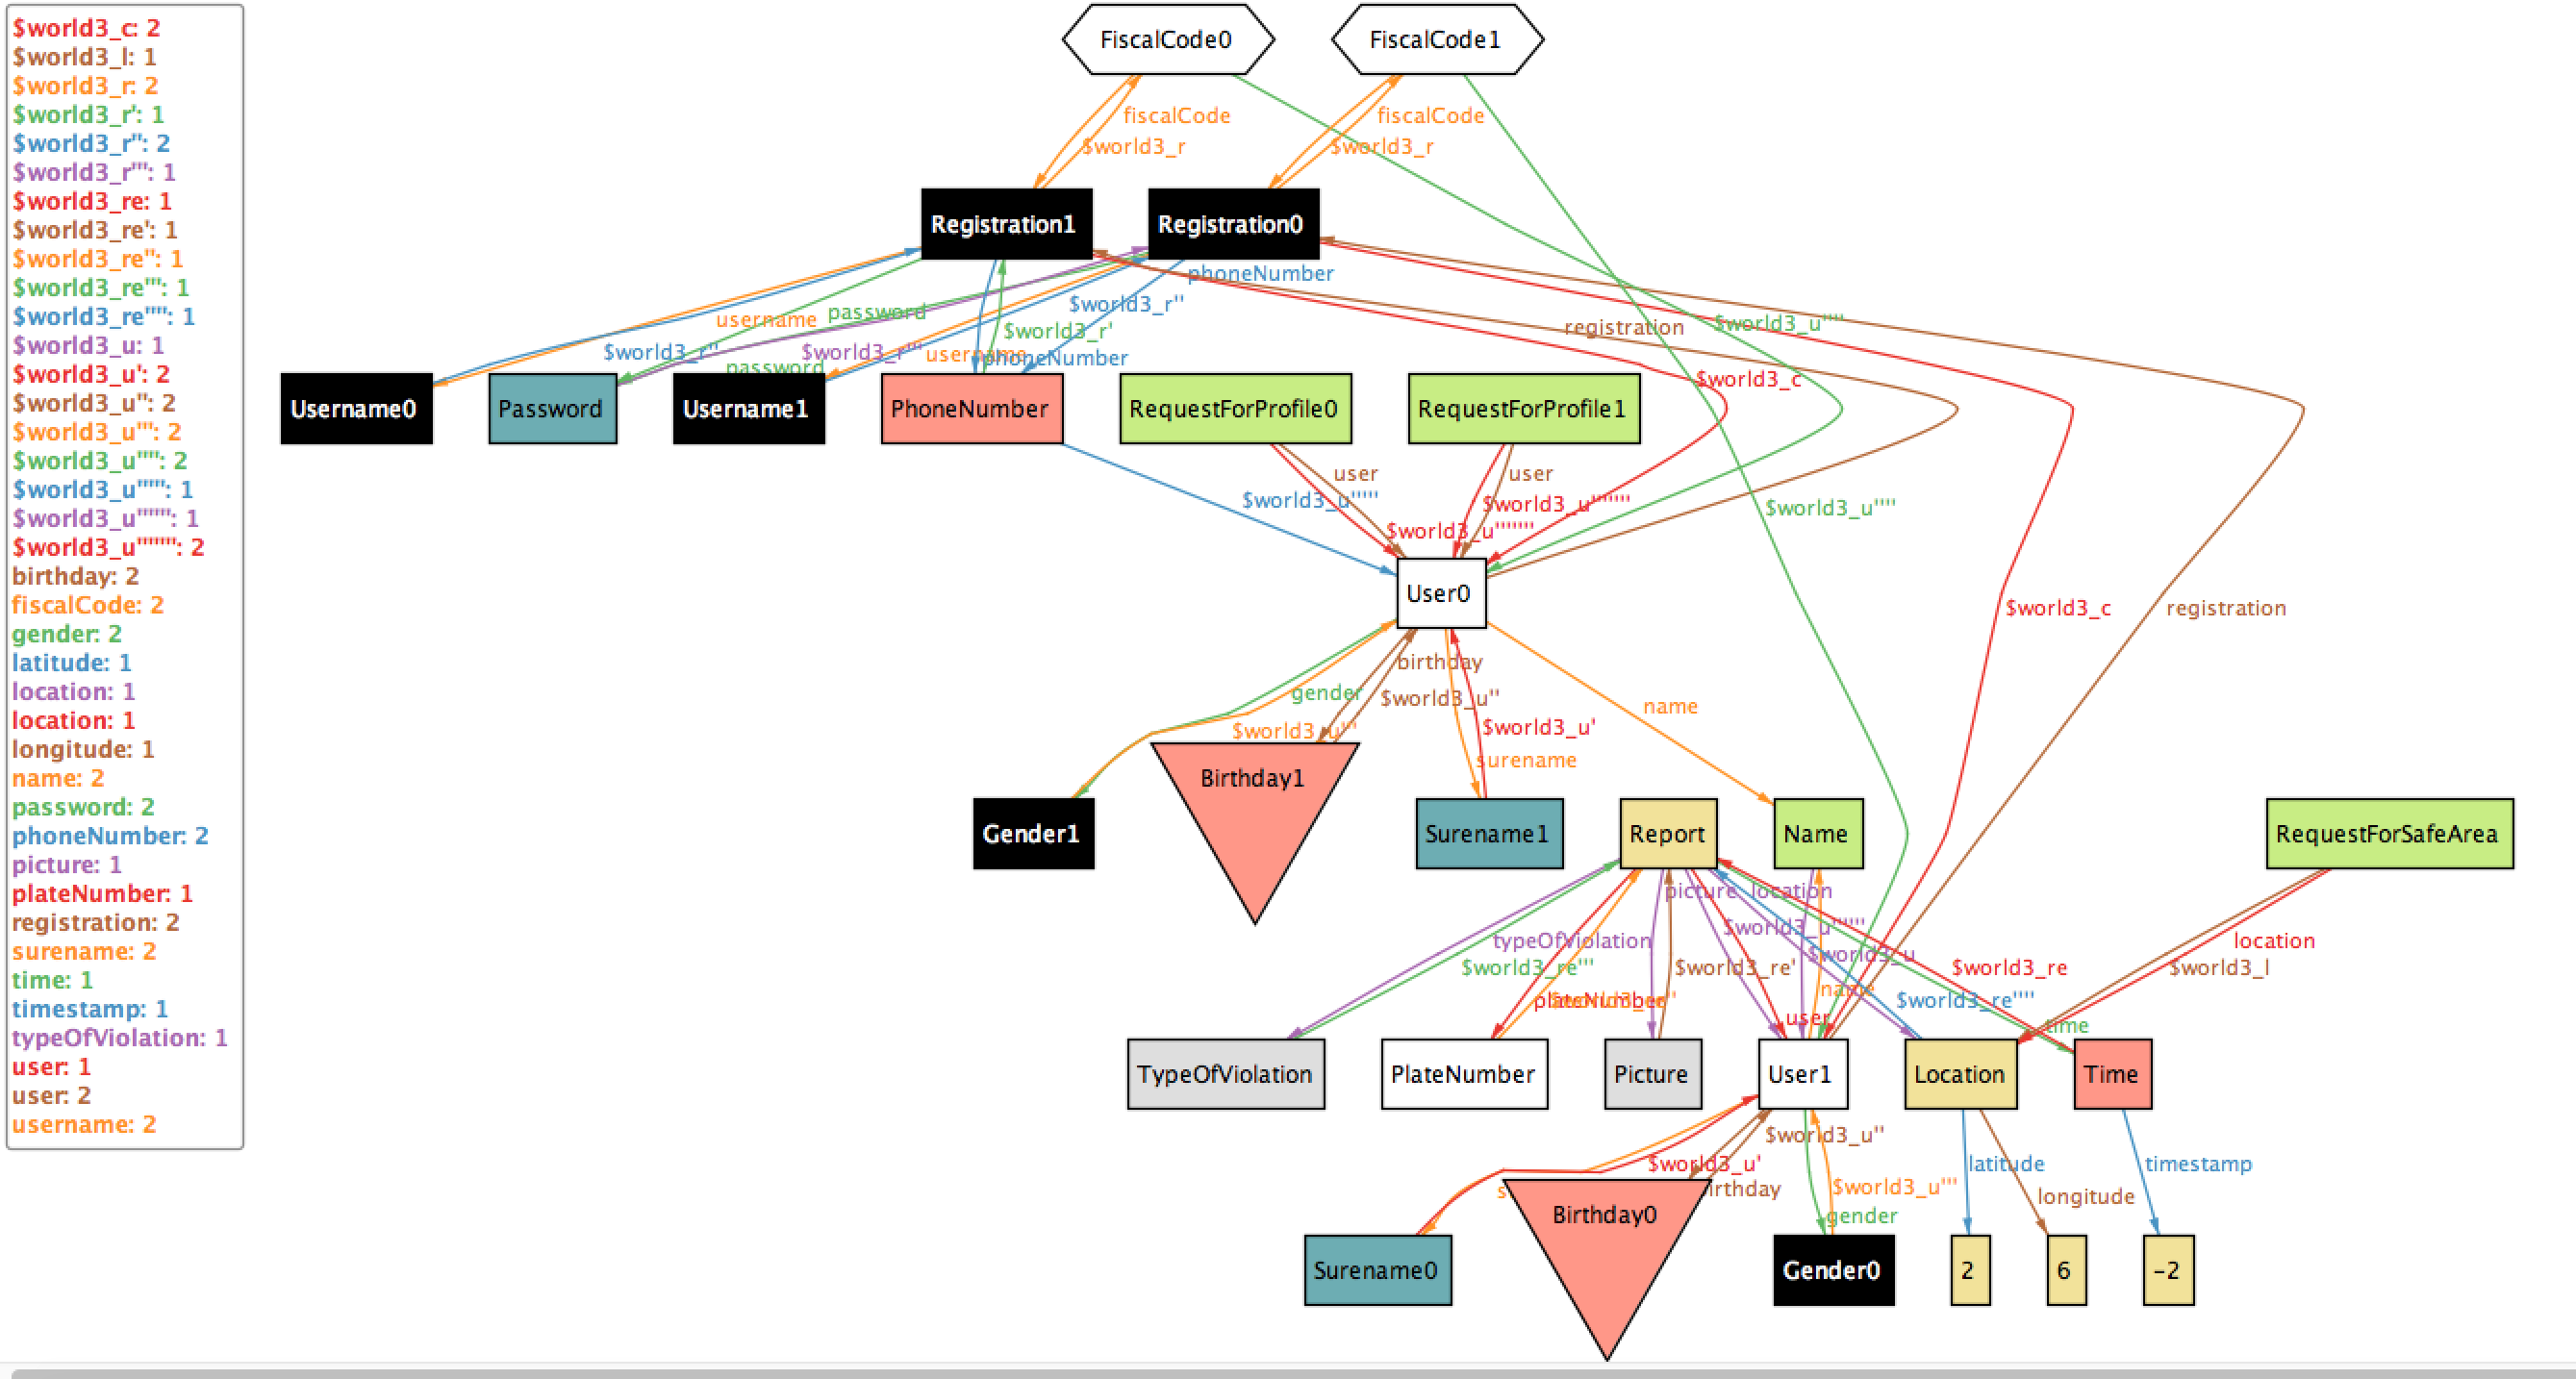
\includegraphics[scale=0.35]{images/World3.png}
		\caption{World Three generated by Alloy Analyzer 4.2}
	\end{figure}
	
The last of the worlds generated in the figure above aims at the consistency of the general functions modeled in the analysis. Specifically, the area safety and profile requests. As seen in the figure, all profile requests must be performed by a single unique user; as well as, the fact that a request to view the safety of a certain area must specify the location in order to be used to find matching reports.


	\begin{figure}[H]	
		\centering
		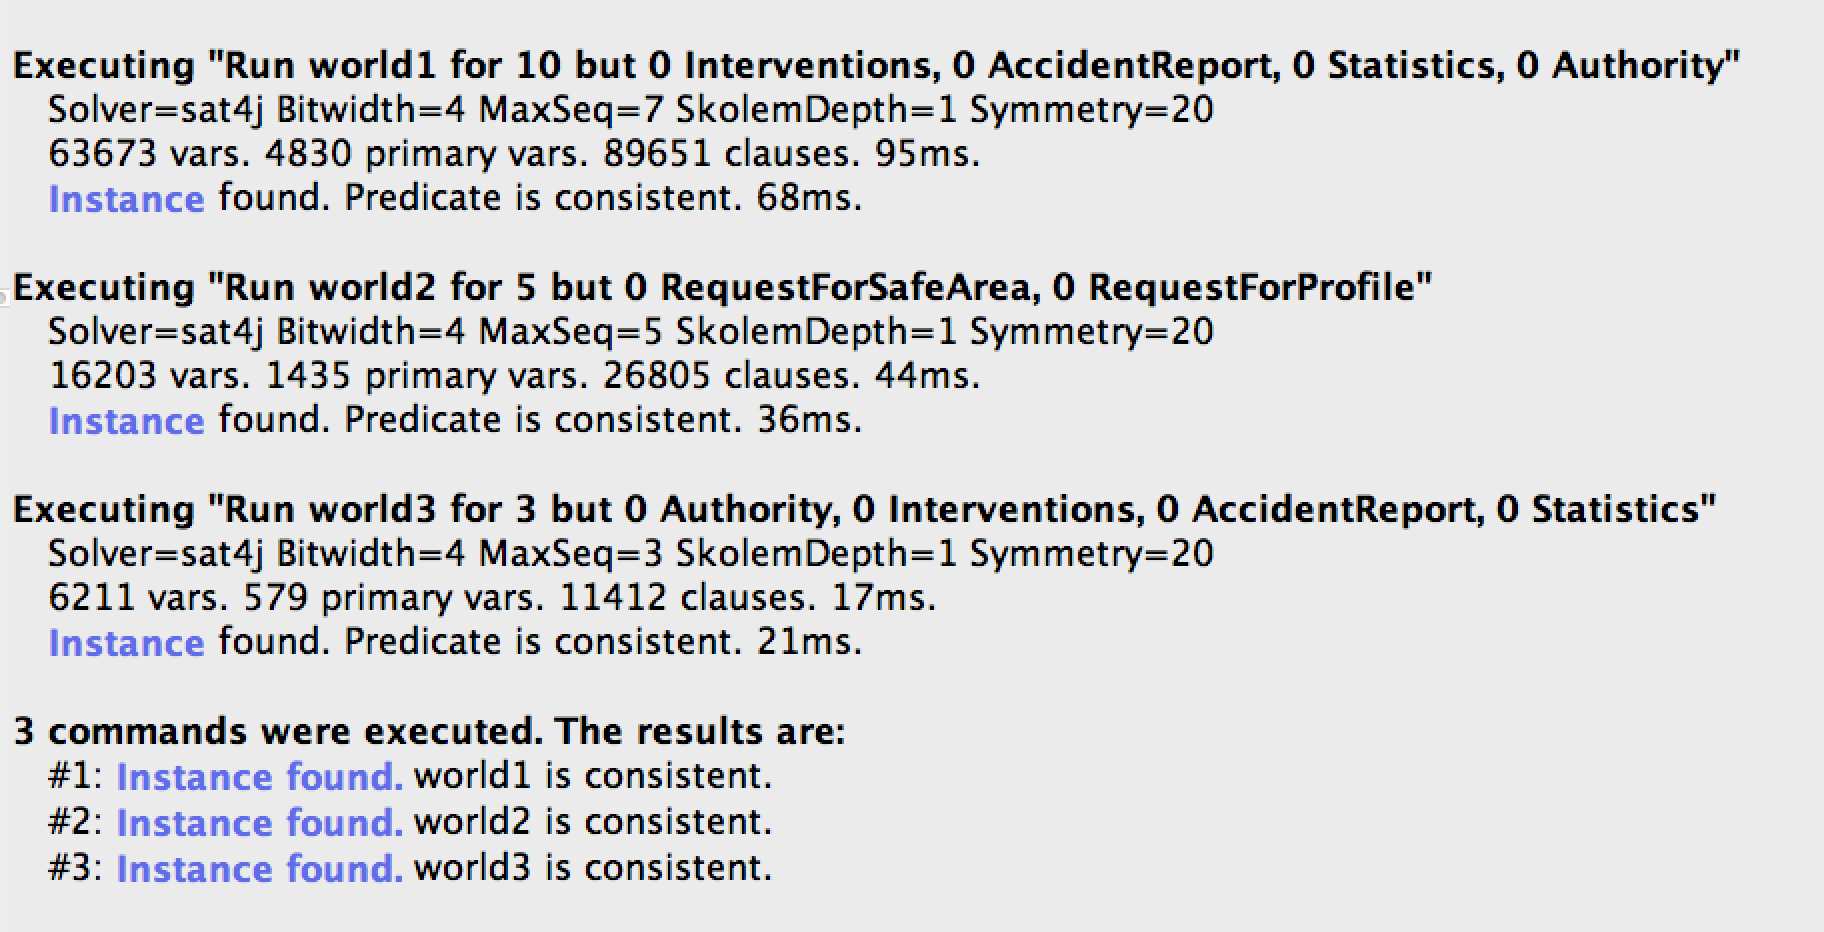
\includegraphics[scale=0.35]{images/Result.png}
		\caption{Result of Worlds generated by Alloy Analyzer 4.2}
	\end{figure}
